\section{Kopiowanie zachowań - wyniki}\label{bc_results}
Metoda \textit{kopiowania zachowań} stanowi punkt wyjściowy i punkt odniesienia dla pozostałych metod.

Nauka agenta sprowadza się do nauczenia klasyfikatora (sieci neuronowej) na podstawie zestawu danych treningowych, czyli zapamiętanych trajektorii eksperta.


\subsection {Zachowanie eksperta}
Podczas prezentacji ekspert zachowuje się tak, jak zachowywałby się człowiek podczas normalnej gry. Działa na podstawie aktualnie widzianego stanu i pamięci na temat poprzednio odwiedzonych stanów (np. pamięta, że poza polem widzenia agenta został niezabity przeciwnik, lub że za rogiem labiryntu zostały niezebrane apteczki). W szczególności ekspert:
\begin{itemize}
\item{w scenariuszu \textit{Trudne zbieranie apteczek} wraca od regionów, w których zostały pominięte wcześniej apteczki}
\item{w scenariuszu \textit{Trudne zbieranie apteczek} znajdując się w rogu lub na ciasnym zakręcie wychodzi z zakrętu na podstawie zapamiętanego wcześniej kierunku ruchu}
\item{w scenariuszu \textit{Trudne zbieranie apteczek} ignoruje apteczki, jeżeli uważa że nie opłaca się ich zbierać}
\item{w scenariuszu \textit{Obrona środka} wbrew optymalnej taktyce okazyjnie strzela do odległych przeciwników}
\item{W scenariuszu \textit{Obrona środka} odwraca się przeciwników, którzy nie są już widoczni na ekranie}
\end{itemize}


\subsection{Wyniki}

Przy testowaniu scenariusza \textit{Obrona środka} dla każdej konfiguracji zostało nauczonych 10 agentów, z których każdy został przetestowany odgrywając 10 epizodów. Wynikowa próbka danych składa się ze 100 wyników dla każdej z konfiguracji.

Przy testowaniu scenariusza \textit{Trudne zbieranie apteczek} dla każdej konfiguracji zostało nauczonych od 82 do 111 agentów, z których każdy został przetestowany odgrywając 20 epizodów. Wynikowa próbka danych składa się z od 1640 do 2220 wyników dla każdej z konfiguracji.

Dla scenariusza \textit{Trudne zbieranie apteczek} wykonano znacznie więcej powtórzeń eksperymentów niż dla \textit{Obrony środka}, żeby upewnić się że różnice pomiędzy algorytmami są statystycznie istotne.

Uczenie sieci przebiega z prędkością około 100 kroków na sekundę, a jego prędkość skaluje się liniowo względem wielkości zestawu danych, tak więc nauka na podstawie trajektorii o rozmiarze 6000 kroków zajmuje około minuty, podobnie jak wykonanie 20 gier testowych.

Maksymalny wynik możliwy do osiągnięcia w scenariuszu \textit{Obrona środka} to 25, a w scenariuszu \textit{Trudne zbieranie apteczek} 2100. Ekspert w większości prezentacji osiąga maksymalne wyniki, ale zdarzają się też wyniki porównywalne z wynikami zaprezentowanymi w tabelach.

W tabelach \ref{tab:simple_expert_results_dtc} i \ref{tab:simple_expert_results_hg} oraz na rysunkach \ref{fig:simple_expert_results_dtc} i \ref{fig:simple_expert_results_hg} przedstawione są wyniki osiągnięte przez agenta w przeprowadzonych eksperymentach.

\begin{figure}[H]
		\ffigbox{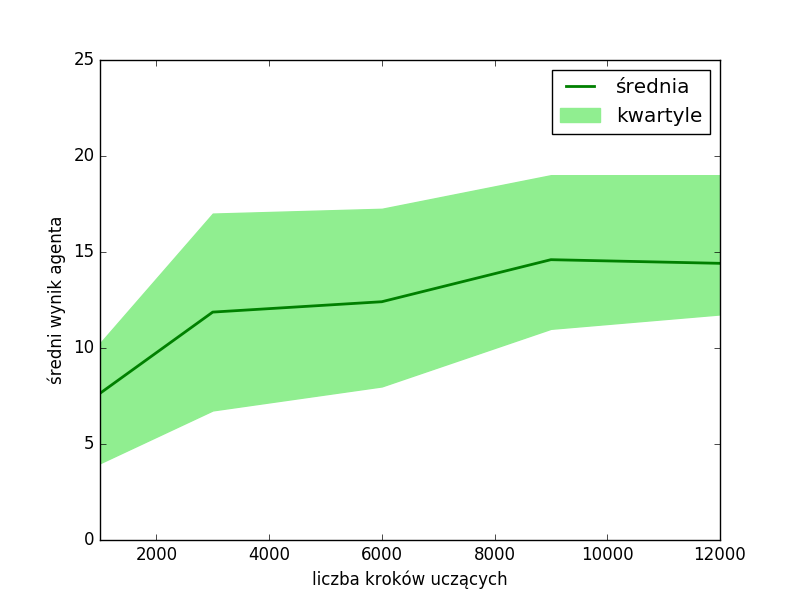
\includegraphics[scale = 0.7]{figures/figures/results/se_dtc_plot.png}}{\caption{Wyniki agenta nauczonego na podstawie trajektorii \textit{zwykłego eksperta} w zależności od liczby kroków uczących w scenariuszu \textit{Obrona środka}}\label{fig:simple_expert_results_dtc}}
\end{figure}

\begin{figure}[H]
		\ffigbox{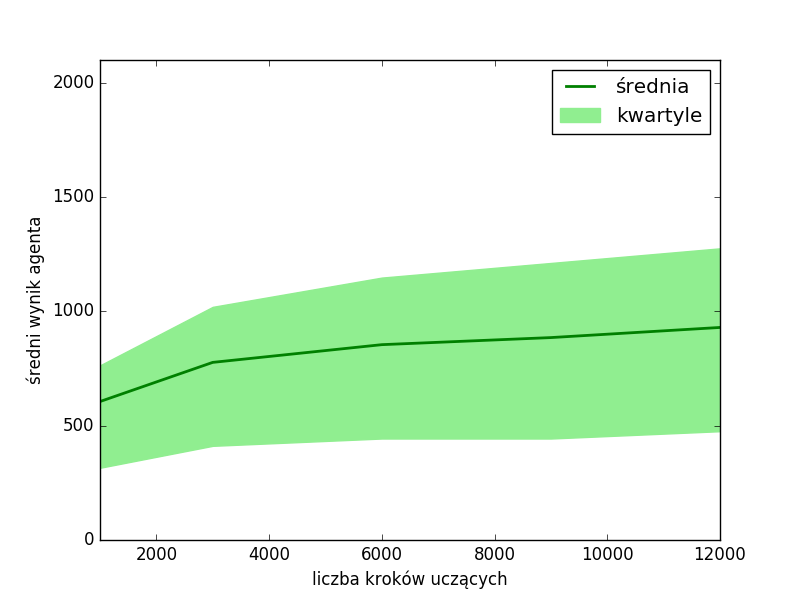
\includegraphics[scale = 0.7]{figures/figures/results/se_hg_plot.png}}{\caption{Wyniki agenta nauczonego na podstawie trajektorii \textit{zwykłego eksperta} w zależności od liczby kroków uczących w scenariuszu \textit{Trudne zbieranie apteczek}}\label{fig:simple_expert_results_hg}}
\end{figure}

\begin{figure}[H]
\csvautotabular{data/simple_expert_results_dtc.csv}{\caption{Wyniki agenta nauczonego na podstawie trajektorii \textit{zwykłego eksperta} w zależności od liczby kroków uczących w scenariuszu \textit{Obrona środka}.}\label{tab:simple_expert_results_dtc}}
\end{figure}

\begin{figure}[H]
\csvautotabular{data/simple_expert_results_hg.csv}{\caption{Wyniki agenta nauczonego na podstawie trajektorii \textit{zwykłego eksperta} w zależności od liczby kroków uczących w scenariuszu \textit{Trudne zbieranie apteczek}.}\label{tab:simple_expert_results_hg}}
\end{figure}

\subsection{Zachowanie agenta}
\subsubsection{Trudne zbieranie apteczek}
Agent wykazuje pełną świadomość labiryntu i otoczenia - poprawnie porusza się po labiryncie, nie wchodzi w ściany i nie blokuje się w ślepych zaułkach. Poprawnie identyfikuje apteczki i zazwyczaj zbiera je zgodnie z oczekiwaniami. Agent bywa niedokładny, na przykład przechodzi zbyt daleko od apteczki by ją zebrać. Agent nie omija min, ale zazwyczaj nie wchodzi w nie z premedytacją. Agentowi zdarza się zablokować pomiędzy dwoma równorzędnymi decyzjami - agent wykonuje wtedy ,,rezonujące'' ruchy (na zmianę wykonuje akcje ,,lewo'' i ,,prawo'' bez ruszania się z miejsca). Najczęściej zdarza się to, gdy agent zajdzie do rogu i nie może zdecydować, w którą stronę powinien się obracać, żeby z niego wyjść.

Agent podczas poruszania się prosto często rozgląda się w lewo i w prawo - jest to artefakt i skutek uboczny wynikający z faktu, że na względnie otwartej przestrzeni wszystkie ruchy są potencjalnie dobre i jedynie szczegóły stanu, takie jak np. rozlokowanie apteczek decyduje o tym, gdzie najbardziej opłaca się udać. W praktyce jest to bardzo pomocne zachowanie, ponieważ przy rozglądaniu się agent może zauważyć korzystne do odwiedzenia obszary.

Polityka zbierania apteczek przez agenta jest najczęściej wystarczająco skuteczna, ale daleka od optymalnej. Agent często skupia się na arbitralnie wybranej apteczce, ignorując apteczki które są bliższe, ale nie ustawione centralnie przed nim. Agent często wybiera też pojedyncze apteczki zamiast zyskownych skupisk apteczek.

\subsubsection{Obrona środka}
Agent rozumie zasady rządzące środowiskiem i zachowuje się poprawnie. Popełnia sporadyczne błędy ignorując przeciwników albo strzelając w pustą przestrzeń. Agent bywa niedokładny, strzelając obok przeciwników. Strategia decydowania o strzelaniu bądź pozostawieniu danego przeciwnika nie jest optymalna. Agent regularnie traci zainteresowanie przeciwnikami, którzy po początkowym nietrafieniu agenta znaleźli się po stronie przeciwnej do obrotowego ruchu agenta. Agent zazwyczaj potrafi rozpoznać, że jest atakowany i obraca się szybko szukając bezpośredniego zagrożenia. Niestety często reakcja występuje zbyt późno.

W zachowaniu agenta nie ma wyraźnych błędów taktycznych, a jedynie niedokładności wyglądające na błędy klasyfikatora.

\subsection{Analiza i wnioski}
Nauczony agent mimo popełnianych błędów zachowuje się poprawnie. Jego zachowanie jest dalekie od optymalnego, ale udało mu się dobrze opanować wszystkie reguły rządzące środowiskiem, w którym się znajduje, oprócz zrozumienia idei min.

Biorąc pod uwagę, jak mało czasu i danych potrzebne było do wytrenowania agenta i porównując jego zachowanie i czas uczenia z zachowaniem i czasem uczenia agenta opisanego w pracy \cite{DBLP:journals/corr/KempkaWRTJ16} można stwierdzić, że metoda \textit{kopiowania zachowań} jest bardzo potężnym narzędziem. 

W scenariuszu \textit{Trudne zbieranie apteczek} agent nie zwraca zazwyczaj uwagi na miny, a wejście w kilka min pod rząd jest najczęstszą przyczyną śmierci agenta. Konstrukcja scenariusza jest taka, że nawet przy mniej efektywnej taktyce zbierania apteczek agent mógłby przeżyć cały epizod, dlatego w praktyce częstotliwość wchodzenia w miny (i w mniejszym stopniu zakleszczania się w rogu labiryntu) jest czynnikiem determinującym średnie wyniki agenta. Warto zauważyć, że tego problemu nie udało się również wyeliminować w pracy \cite{DBLP:journals/corr/KempkaWRTJ16}.
